
\documentclass[
12pt,
a4paper,
pdftex,
czech,
titlepage
]{report}

\usepackage{float}
\usepackage[czech]{babel}
\usepackage[utf8]{inputenc}
\usepackage{lmodern}
\usepackage{textcomp}
\usepackage[T1]{fontenc}
\usepackage{amsfonts}
\usepackage{titlesec}
\usepackage{graphicx}
\usepackage{longtable}
\usepackage{multirow}
\usepackage{tabularx} 
\usepackage[unicode]{hyperref}
\usepackage{indentfirst}
\hypersetup{
    colorlinks=true,
    citecolor=green,
    filecolor=black,
    linkcolor=black,
    urlcolor=magenta
}
\titleformat{\chapter}
  {\normalfont\LARGE\bfseries}{\thechapter}{1em}{}
\titlespacing*{\chapter}{0pt}{0ex plus 1ex minus .2ex}{2.0ex plus .2ex}



\begin{document}

\begin{titlepage}
	\vspace*{-2cm}
	{\centering
\includegraphics[scale=1.5]{FAV_logo.pdf}\par}
	\centering
	\vspace*{2cm}
	{\Large Dokumentace k semestrální práci z KIV/PIA\par}
	\vspace{1.0cm}
	{\Huge\bfseries KIVBOOK\par}
	\vspace{7cm}

	\begin{flushleft} 
	\begin{table}[ht]
	\label{stats}
	\begin{tabular}{ll}
	\textbf{Student:}  & Martin Kružej   \\
	\textbf{St. číslo:}   & A17N0079P    \\
	\textbf{E-mail:}  & kruzej@students.zcu.cz  \\
	\textbf{Datum:}    & \today            \\ 
	\end{tabular}
	\end{table}
	\end{flushleft}
	
	\vfill


\end{titlepage}

\tableofcontents
\thispagestyle{empty}
\clearpage

\chapter{Zadání}
\setcounter{page}{1}

Standardní téma KIV/PIA, viz \href{https://courseware.zcu.cz/portal/studium/courseware/kiv/pia/samostatna-prace/standardni-tema.html}{KIV/PIA courseware}.

\chapter{Architektura aplikace}

\section{Obecná architektura}

Aplikace je postavená na technologii Java EE. Jednoduchý diagram ukazující základní obecný chod aplikace je uveden na diagramu \ref{general}. Uživatel pracuje s tzv. front-endme, který je na klientovi ve formě HTML a CSS. Při zaslání požadavku je tento požadavek předán tzv. back-endu. Zde je zpracován jedním ze servletů, ti v případě potřeby mohou volat databázi přes třídy Manažerů a Dao. Poté vyberou některý z JSP souborů dle požadavku a ten vrací zpět na front-end, kde je zobrazen již ve formátu HTML a CSS. K architektuře bude řečeno více detailů v následujících kapitolách.

\begin{figure}[H]
\caption{Obecná architektura}
\label{general}
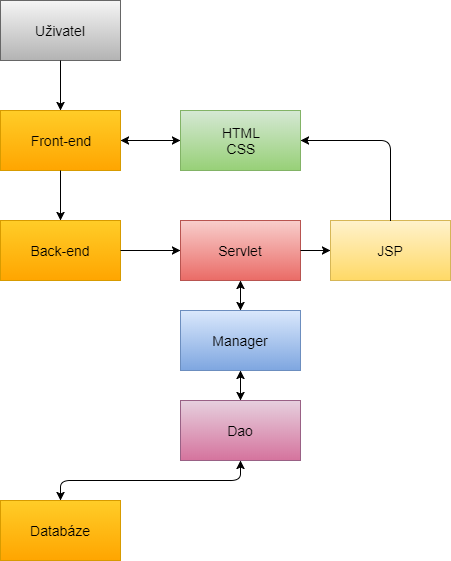
\includegraphics[width=\textwidth]{general.png}
\end{figure}

\section{Architektura servletů}

Servlety jsou základní kámen serveru - tyto servlety obsluhují veškeré požadavky, které na server chodí. Pro přístup k databázi využívají různé manažery a tyto manažery jim musí někdo poskytnout. Máme zde třídu ApplicationContext, která vytvoří všechny potřebné třídy Manažerů a Dao. Při inicializaci je spuštěn StartupListener, který třídy z ApplicationContext injekčně dopraví do servletů, které to potřebují. Tento styl se často označuje jako \textit{Dependency injection}. 

Při vyslání požadavku na server se tento požadavek nedostane k servletům hned. Nejdříve projde EncodingListener, jenž zajišťuje kódování charakterů ve formátu UTF-8. Dále jsou určité servlety za jakousi bránou, která je brání před neautorizovaným přístupem. Tato brána je AuthenticationGuard využívající AuthenticationService. Tyto dvě třídy pouze kontrolují, že pro přístup k některým servletům je třeba být přihlášen.

Diagram znázorňující tuto architekturu je uveden na obrázku \ref{servlety}.

\begin{figure}[H]
\caption{Architektura servletů}
\label{servlety}
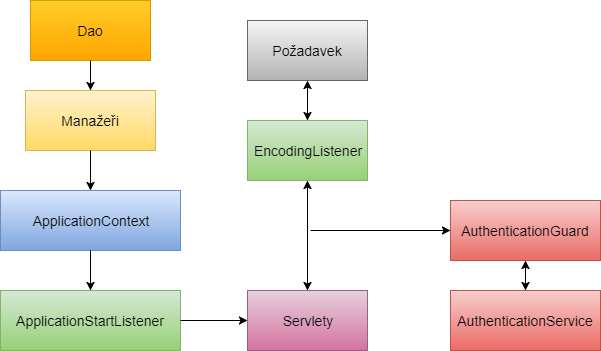
\includegraphics[width=\textwidth]{servlety.png}
\end{figure}

\section{Architektura entit}
Před podíváním o Manažerech je třeba se podívat na nejnižší úroveň této architektury a to jsou entity. Tyto entity jsou v podstatě tabulky, které se v databázi používají. Nejdříve je zde rozhraní IEntity, které dědí abstraktní třída BaseEntity. Tyto dvě třídy poskytují jednotné \textit{id} pro všechny entity. Ty existují následující:
\begin{itemize}
\item \textbf{User} - uživatel v databázi
\item \textbf{Status} - status/tweet v databázi
\item \textbf{Friendship} - přátelství / požadavek na přátelství v databázi
\end{itemize}

Následuje dědění abstraktní třídy entitami. Tento vztah je vyobrazen na obrázku \ref{entity}.

\begin{figure}[H]
\caption{Architektura entit}
\label{entity}
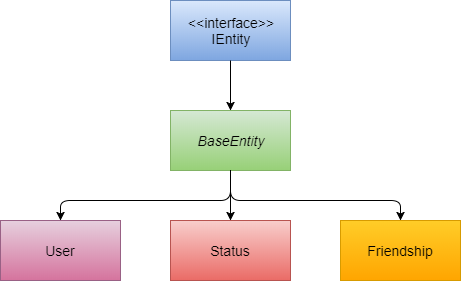
\includegraphics[width=\textwidth]{entity.png}
\end{figure}

\section{Architektura Manažerů}
Manažeři mají za úkol poskytnout prostředníka mezi servlety a databází, potažmo Dao. Poksytují různé metody pro práci s databází či entitami. Opět se zde setkáváme s rozhraními, ze kterých jsou potom odvozeny samotné třídy. Pro každou jednotlivou entitu existuje jednotliví Manažer. Servlety obecně pracují právě s rozhraním, které je jim injektováno a již je jim jedno, jakou implementaci Manažerů používají.

Vyobrazeno na obrázku \ref{manazeri}.

\begin{figure}[H]
\caption{Architektura Manažerů}
\label{manazeri}
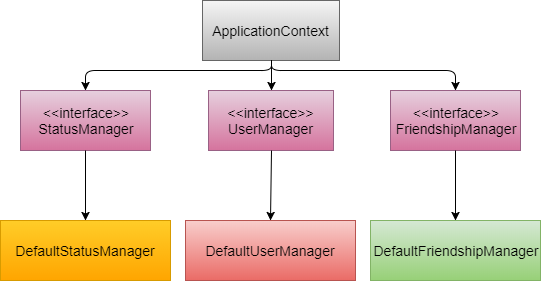
\includegraphics[width=\textwidth]{manazeri.png}
\end{figure}

\section{Architektura Dao}
Tato úroveň pracuje s databází. Přes rozhraní slibuje různé metody pro tuto práci a poté je i implementuje. Vzhledem k tomu, jak je tato architektura navržena, je možno udělat několik různých implementací těchto Dao tříd. V aplikaci je použito Criteria, ale je možno udělat třeba JPQL pouhým přidáním tříd a změnou injektování. 

Základní rozhraní je GenericDao, kde se definují ty nejzákladnější metody, které každé Dao musí implementovat - jako najít instanci, uložit instanci, smazat instanci. Toto rozhraní dědí rozhraní deklarující již specifické metody pro různé entity - FriendshipDao, UserDao a StatusDao. Tyto třídy jsou to rozhraní, které je injektováno třídou ApplicationContext.

Následuje specifikace JPA. Nejdříve obecná třída GenericDaoJpa s velice obecnými metodami. Následují abstraktní třídy pro jednotlivé entity. Tyto třídy dědí jak GenericDaoJpa tak jednotlivé Dao rozhraní. Poslední částí architektury jsou samotné implementace jednotlivých metod. Jak bylo řečeno v předešlých odstavcích, tato aplikace využívá Criteria, ale zde by mohly být další třídy, např. FriendshipDaoJPQL využívající JPQL. 

Vyobrazeno na obrázku \ref{dao}.

\begin{figure}[H]
\caption{Architektura Dao}
\label{dao}
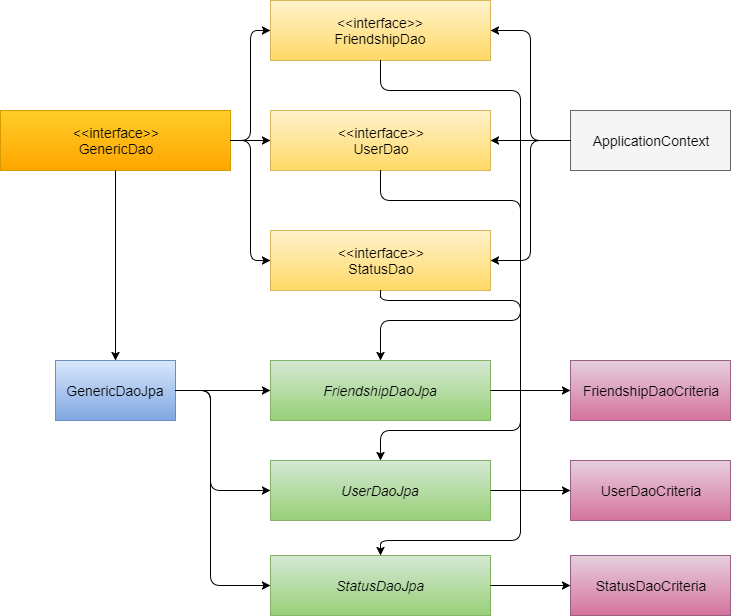
\includegraphics[width=\textwidth]{dao.png}
\end{figure}

\chapter{Aplikace}

\section{Use case}

Aplikace imituje některé známé sociální sítě. Use case aplikace je vyobrazen na obrázku \ref{use_case}.
Horní část diagramu ve světlé žluté je ta část, která je přístupná nepřihlášenému uživateli. Tento uživatel si může prohlížet některé statické stránky, seznam registrovaných uživatelů a profily těchto uživatelů. Přístup ke zbytku aplikace mu bude zamítnut dokud se nezaregistruje/nepřihlásí.

Po přihlášení do systému je uživateli zpřístupněn zbytek aplikace. Dostává nyní vlastní zeď, může upravovat svůj profil, dívat se na své přátele, žádat o přátelství, zamítat přátelství a také vytvářet statusy a lajkovat/hejtovat je. 

\begin{figure}[H]
\caption{Use case}
\label{use_case}
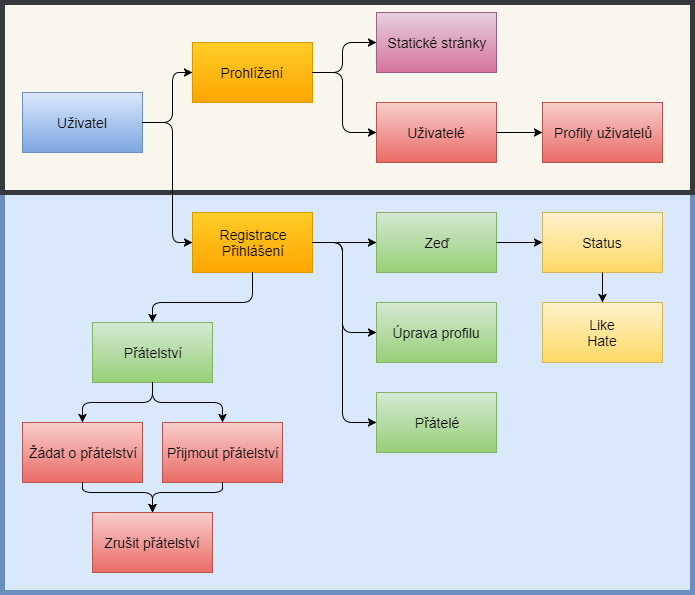
\includegraphics[width=\textwidth]{use_case.png}
\end{figure}

\section{Prohlížení stránek}

Aplikace podporuje nepřihlášenému uživateli prohlédnout si některé stránky. Může se podívat na názory některých uživatelů či informace o aplikaci. Je mu dovoleno zhlédnout seznam registrovaných uživatelů a může si prohlížet jejich profily. Sám nikde nenajde nikdy odkaz, který by ho zavedl do privilegované části aplikace, ale chytrý uživatel může samozřejmě měnit URL. Proto je v aplikaci AuthenticationGuard, který nepřihlášeného uživatele nikam dál nepustí a vybídne ho k přihlášení.

\section{Registrace}

Uživatel má možnost se zaregistrovat. Bude mu nabídnut registrační formulář s následujícími položkami:
\begin{itemize}
\item \textbf{Uživatelské jméno} - uživatelovo jméno, kterým se bude přihlašovat - \textbf{povinné}
\item \textbf{Heslo} - heslo k uživatelskému účtu - \textbf{povinné}
\item \textbf{Kontrola hesla} - znovu zadání hesla - \textbf{povinné}
\item \textbf{Pohlaví} - jestli je uživatel muž, či žena - \textbf{nepovinné}
\item \textbf{Datum narození} - kdy se uživatel narodil - \textbf{nepovinné}
\item \textbf{Souhlas s podmínkami} - uživatel souhlasí s podmínkami - \textbf{povinné}
\item \textbf{Kontrola robotů} - uživatel je nucen napsat číslici 4 - \textbf{povinné}
\end{itemize}

Povinné položky formulář nepovolí odeslat, dokud nejsou vyplněny. Uživatelské jméno je povoleno pouze písmena a číslice. Hesla se musejí shodovat. Datum narození nemusí být vyplněn vůbec ale pokud uživatel vyplní pouze část data, je mu vynadáno. Heslo je dále hashováno, než je uloženo do databáze. V případě chybných údajů, například že se neshodují hesla, je formulář předvyplněn některými údaji, jmenovitě uživatelské jméno, pohlaví, souhlas s podmínkami a kontrola robotů.

\section{Přihlášení}

Při přihlášení uživatel vyplňuje svoje uživatelské jméno a heslo. V případě neshody je uživatel nepřihlášen. Po úspěšném přihlášení se schovávají položky pro přihlášení/registraci a jsou nahrazeny profilem a odhlášením. Nyní je uživatel volný kamkoliv do aplikace. Žádný odkaz nevede zpátky do statických stránek, ale chytrý uživatel si samozřejmě poradí. Pokud se přihlášený uživatel dostane zpět na stránky registrace a přihlášení, jednoduše mu nebude dovoleno žádnou z forem vyplňovat, dokud bude přihlášen.

\section{Prohlížení uživatelů}



\end{document}